%%%%%%%%%%%%%%%%%%%%%%%%%%%%%%%%%%%%%%%%%
% Journal Article
% LaTeX Template
% Version 1.4 (15/5/16)
%
% This template has been downloaded from:
% http://www.LaTeXTemplates.com
%
% Original author:
% Frits Wenneker (http://www.howtotex.com) with extensive modifications by
% Vel (vel@LaTeXTemplates.com)
%
% License:
% CC BY-NC-SA 3.0 (http://creativecommons.org/licenses/by-nc-sa/3.0/)
%
%%%%%%%%%%%%%%%%%%%%%%%%%%%%%%%%%%%%%%%%%

%----------------------------------------------------------------------------------------
%	PACKAGES AND OTHER DOCUMENT CONFIGURATIONS
%----------------------------------------------------------------------------------------

\documentclass[twoside,twocolumn]{article}

\usepackage{blindtext} % Package to generate dummy text throughout this template 

\usepackage[sc]{mathpazo} % Use the Palatino font
\usepackage[T1]{fontenc} % Use 8-bit encoding that has 256 glyphs
\linespread{1.05} % Line spacing - Palatino needs more space between lines
\usepackage{microtype} % Slightly tweak font spacing for aesthetics

\usepackage[english]{babel} % Language hyphenation and typographical rules

\usepackage[hmarginratio=1:1,top=32mm,columnsep=20pt]{geometry} % Document margins
\usepackage[hang, small,labelfont=bf,up,textfont=it,up]{caption} % Custom captions under/above floats in tables or figures
\usepackage{booktabs} % Horizontal rules in tables

\usepackage{lettrine} % The lettrine is the first enlarged letter at the beginning of the text

\usepackage{enumitem} % Customized lists
\setlist[itemize]{noitemsep} % Make itemize lists more compact

\usepackage{abstract} % Allows abstract customization

\usepackage{graphicx}
\graphicspath{ {images/} }

\renewcommand{\abstractnamefont}{\normalfont\bfseries} % Set the "Abstract" text to bold
\renewcommand{\abstracttextfont}{\normalfont\small\itshape} % Set the abstract itself to small italic text

\usepackage{titlesec} % Allows customization of titles
\renewcommand\thesection{\Roman{section}} % Roman numerals for the sections
\renewcommand\thesubsection{\roman{subsection}} % roman numerals for subsections
\titleformat{\section}[block]{\large\scshape\centering}{\thesection.}{1em}{} % Change the look of the section titles
\titleformat{\subsection}[block]{\large}{\thesubsection.}{1em}{} % Change the look of the section titles

\usepackage{fancyhdr} % Headers and footers
\pagestyle{fancy} % All pages have headers and footers
\fancyhead{} % Blank out the default header
\fancyfoot{} % Blank out the default footer
\fancyhead[C]{EN 600.461: Computer Vision $\bullet$ December 2016 } % Custom header text
\fancyfoot[RO,LE]{\thepage} % Custom footer text

\usepackage{titling} % Customizing the title section

\usepackage{hyperref} % For hyperlinks in the PDF

%----------------------------------------------------------------------------------------
%	TITLE SECTION
%----------------------------------------------------------------------------------------

\setlength{\droptitle}{-4\baselineskip} % Move the title up

\pretitle{\begin{center}\Huge\bfseries} % Article title formatting
\posttitle{\end{center}} % Article title closing formatting
\title{SmartWall} % Article title
\author{%
\textsc{Gary Qian, Manyu Sharma, Sarah Sukardi, Tony Jiang}\\[1ex] % Your name
\normalsize Johns Hopkins University, Department of Computer Science \\ % Your institution
%\normalsize \href{mailto:john@smith.com}{john@smith.com} % Your email address
%\and % Uncomment if 2 authors are required, duplicate these 4 lines if more
%\textsc{Jane Smith}\thanks{Corresponding author} \\[1ex] % Second author's name
%\normalsize University of Utah \\ % Second author's institution
%\normalsize \href{mailto:jane@smith.com}{jane@smith.com} % Second author's email address
}


\date{\today} % Leave empty to omit a date
\renewcommand{\maketitlehookd}{%
\begin{abstract}
\noindent 
This paper presents Smartwall, a program that uses computer vision to turn any surface into an interactive board using a standard camera (such as a webcam) and a projector. The program uses a custom calibration matrix and perspective projection to enable object tracking, as well as employs deep learning for hand recognition and gestural board manipulation. Smartwall is an extremely accurate, cost-effective, and simple way to facilitate interactive teaching, brainstorming, and entertainment, at a fraction of the cost of other existing devices.
\end{abstract}
}

%----------------------------------------------------------------------------------------

\begin{document}

% Print the title
\maketitle

%----------------------------------------------------------------------------------------
%	ARTICLE CONTENTS
%----------------------------------------------------------------------------------------

\section{Introduction}

\lettrine[nindent=0em,lines=3]{H} umans have drawn on surfaces for millenia. From primitive pre-historic cave paintings to 17th century frescoes to the chalkboards and whiteboards commonly used in schools and universities today, the usage of surfaces as conduits for brainstorming, depicting information, and even art, have made them long essential to processes of creativity and conveyance.\\ \\Current, modern approaches to drawing on surfaces suffer from either requiring physical, depletable media (whiteboards, chalkboards, pens, paint) or expensive equipment (modern-day smartboards, MSRP ~\$1000 - \$9000). This paper presents a cost-effective method to turn any wall into a drawable surface (and more generally, full computer control) using only two pieces of equipment: a camera and a projector, where the projector can be substituted with any medium capable of displaying digital content (ie. televisions, monitors, etc.). The camera requirement can be filled by readily available webcams present on almost all modern laptops.\\ \\ Our method is easily adaptable to spaces with unique constraints and requires equipment that most modern rooms already come equipped with, combining both traditional as well as state-of-the art computer vision techniques to allow for sophisticated and accurate gestural recognition.
%------------------------------------------------
\section{Methods}

We separate our discussion of methods into several subsections:
\begin{itemize}
\item Calibration
\item Detection
\item Training
\item Recognition
\item Output
\end{itemize}
\subsection{Calibration}

\begin{center}
	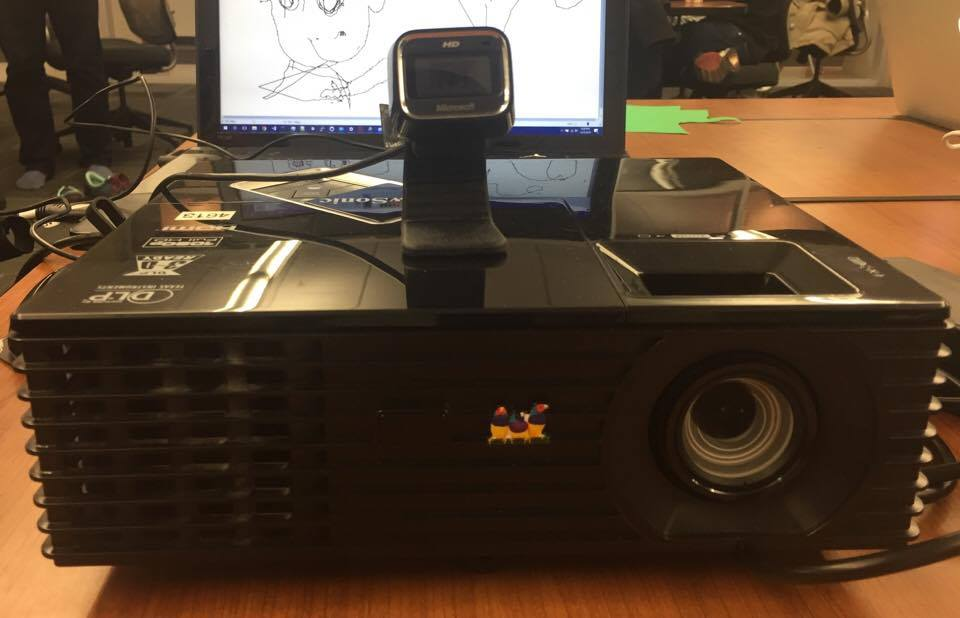
\includegraphics[scale=0.19]{setup} \\
	\vspace{0.25cm}
	\small{\textbf{Figure 1:} \textit{Sample Setup with Camera and Projector}}
\end{center}

For camera calibration, the camera used to track hand movement is set to point towards the wall. Note: we will proceed to use the phrase projector to represent any display medium from TV screens to actual projectors. The projector projects the content eventually to be controlled with a human hand in the same direction as the camera. A custom pattern of green dots is displayed onto the wall for the camera to record; this is the setup required for the camera calibration process to begin. The pattern we found that worked the best was 9 green dots arranged in a x pattern as shown. This pattern results in full coverage of the extremities of the projected screen, ensuring capture of any strange warping effects. Each dot has a unique x position, which will be used later to sort and match the detected dots with their expected locations. Also, each dot's position and size is relative to the projector resolution, ensuring compatibility with a projector of any size and resolution. This method will work under the assumption that the projection surface will be flat and fully visible to the camera.

\begin{center}
	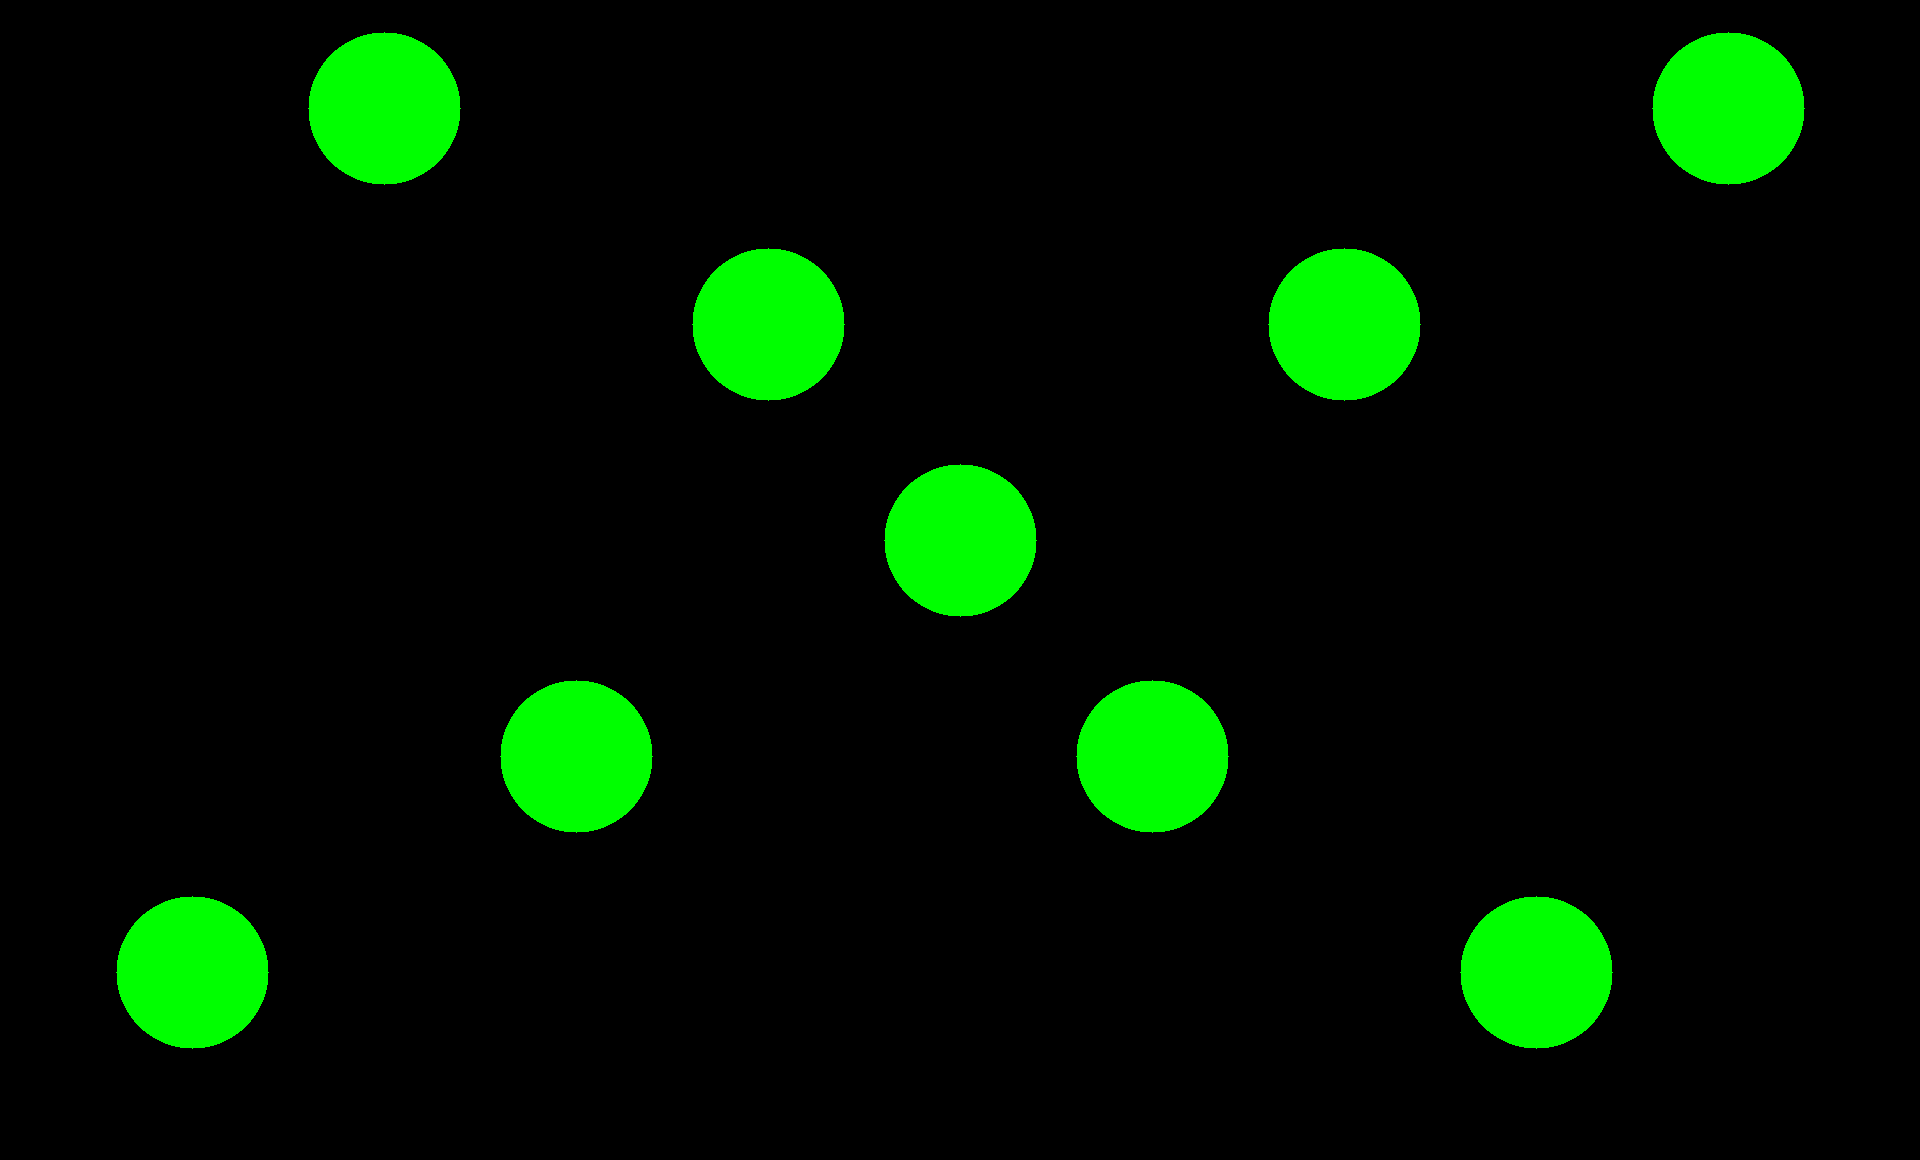
\includegraphics[scale=0.12]{calibrationMatrix} \\
	\vspace{0.1cm}
	\small{\textbf{Figure 2:} \textit{Custom Calibration Matrix}}
\end{center}

The camera then begins the process of calibration. Frames are captured in real-time from the camera. For each frame, a box blur with an 9-pixel diameter is applied to the image (this blur radius is manually adjusted and 9 seemed to work the best; the smaller the radius, the smaller the detectable objects are). Each frame is then converted to HSV color-space to detect hues on the screen. An HSV image can isolate certain colors without regard to the specific saturation or brightness of the patch. The range of color to be detected is then defined manually and thresholded to retrieve a binary image of only the desired colors, where 255 is green areas and 0 is everything else. For calibration, we used green, which was chosen because of the lack of green in skin tones, and the camera's increased green sensitivity due to the Bayer patterns of most cameras today. In the threshold values, we cut off colors that are too unsaturated because at low saturation, the color accuracy is very susceptible to noise. We also cut off areas that are too dark because lowlight performance of cameras is also unreliable. and grainy. Finally, the thresholded mask is eroded to remove noise.\\ \\
From each color isolated frame, contours are drawn around each blob and the center of each contour is computed. We say that often times, a large solid green patch could potentially end up with two or more very close but disconnected blobs representing it. To resolve this, any nearby contour centers within a 30-pixel radius are clustered to form a single point to consolidate any single blob that was broken up due to noise. The amount of detected points from the image is then counted. \\ \\
When the amount of detected points is equal to the amount of points on the custom pattern (in our case, 9) designed for optimum calibration, the points are sorted by x coordinate and matched with the database of known points. Since the points all have unique x positions, we can simply match the lowest x position detected point with the lowest x position known point and so on. We found that this process is actually extremely robust in most conceivable uses and can still reliably match points even under very extreme tilt positions and placement angles of the camera. From the 9 matched point pairs, a homography is found to output a transformation matrix from camera space to projector space. If the pattern is not adequately detected (detected points $\neq$ 9), the system continues the process again for up to a set amount of frames, after which the program will assume that conditions are not adequate and will prompt the user to readjust so that a proper homography can be found.\\ \\
We have found that our system accurately detects our custom pattern projected onto a flat white background in less than 10 iterations, or frames, even with the camera positioned at various angles. In good conditions, the detection will often happen in the first frame. Overall, the detection time often depends on the camera auto-focusing and white balancing, which will depend on each individual camera.\footnote{Source code in provided file \textbf{calibrate.py}.}.

\subsection{Detection}
After camera calibration has occurred, the program switches into real-time capture mode for object detection. After a frame captured real-time is converted to HSV, thresholded, eroded, contoured, and filtered to remove unwanted detections (similar to the algorithm used for initial calibration object detection), the colored point detected is transformed using the projective transformation found during the process of camera calibration to find the corresponding location on the screen. To further filter out invalid points, if the contour center's transformed location is out of range of the screen, it is discarded.\\ \\ Once the location of the detected point in both camera and world coordinates has been found, a point can be directly output onto the screen in the location of the detected point, or the point can be sent for further processing and image recognition. \footnote{Source code in provided file \textbf{display.py}}

\subsection{Training}
Training for subsequent object recognition was performed using the Keras library for Python. Over 7000 images of open and closed hands with variation of skin tones and lighting conditions and with differing backgrounds were captured to accumulate a robust training data set. In captured images, a green square with optimal hue for camera calibration was placed onto the hand; a red dot was then superimposed through software onto the hand to allow for different color recognition and color-agnostic training by the neural network by simply covering up the green patch. Each training image consisted of a 32x32 image. The sample space depends on the resolution of the camera. For example, for a 640x480 webcam, the 32x32 image is created by down-sampling a 64x64 area on the webcam image. For smaller screens, the area represented can be dynamically adjusted.

\begin{center}
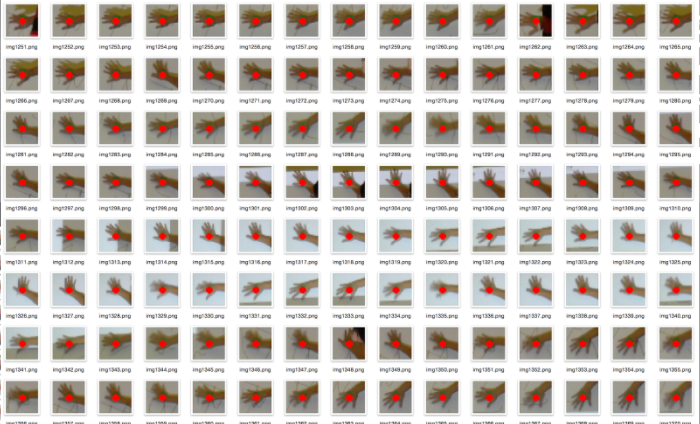
\includegraphics[scale=0.25]{training_data} \\
\vspace{0.25cm}
\small{\textbf{Figure 3:} \textit{Custom Training Data}}
\end{center}

The images obtained were trained against using a deep convolutional neural network, using a pattern of Convolutional, Dropout, Convolutional, and Max Pooling layers repeated 3 times with 32, 64, and 128 feature maps. Finally, a larger Dense layer was used at the output of the convolutional neural network to more efficaciously translate the large number of feature maps to class values. \\ \\
The network topology was defined in Keras and the model trained using 100 epochs and a batch size of 32. This training allowed for subsequent object recognition of open and closed hands with over 99\% accuracy under controlled (typical) conditions.\footnote{Source code in provided file \textbf{recognize.py}}

\subsection{Recognition}
The process of object recognition begins when one point (and only one point) has been detected by the system in real-time. This requirement is enforced due the technical limitation that windows computers only register one mouse pointer. If implemented on a device such as a tablet with multitouch support, multiple points can easily be captured. When only one colored point has been detected, a 32 x 32 pixel window around the detected point is captured (in the same way as the training data) and then sent for processing. It is then input into the deep learning model for classification into one of two trained states: open hand and closed hand. A prediction is generated based on the two output probabilities into one of the two states. \\ \\ To prevent erroneous click events from one or two stray incorrect closed hand prediction states, click events are only sent when two or more previous frames have been predicted by the neural network to be closed-hand frames. This is implemented by retaining a 3 frame buffer, where the majority state (in this case, 2) will determine the current prediction. Only then is the click event deployed by the system. Through experimentation, we found that our classification system was accurate enough that a minimal buffer of 3 was enough to eliminate almost all erroneous clicks while keeping latency down. \footnote{Source code provided in file \textbf{display.py}}

\subsection{Output}

\begin{center}
	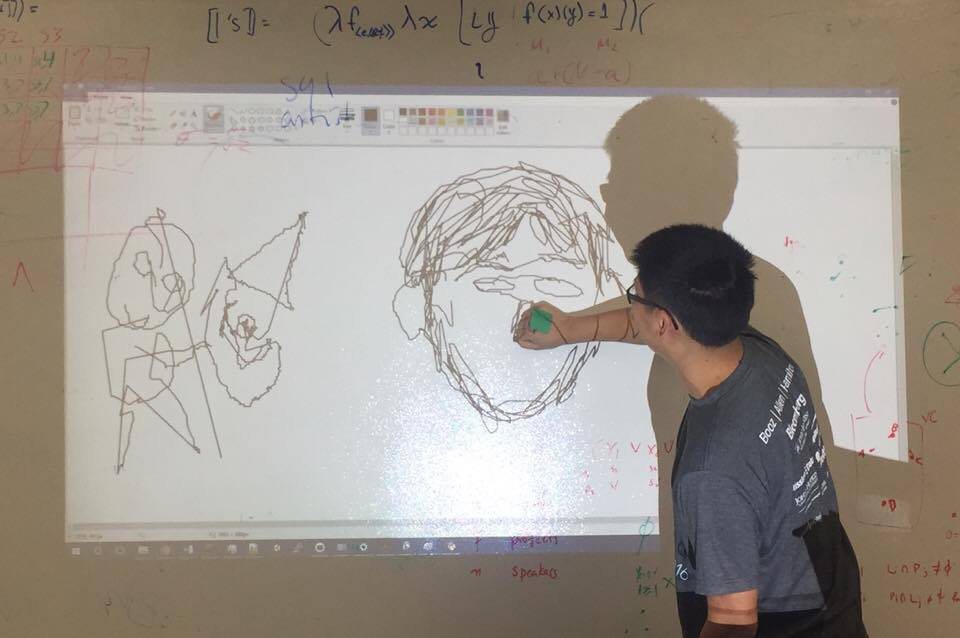
\includegraphics[scale=0.19]{sample} \\
	\vspace{0.25cm}
	\small{\textbf{Figure 4:} \textit{Sample Drawing Made with SmartWall}}
\end{center}

Closed to Open hand gesture transitions are mapped by the system to mouse button up events, and opend to closed hand gesture transitions are mapped to mouse button down events. A drawing system where one can draw onto the screen only upon closed-hand events is built into the system for demonstration purposes. Additionally, a system for controlling the machine running the program using mouse events is also built into the SmartWall system. This system provides the fundamental functionality of what is known as a smartboard of full computer mouse control.
 %------------------------------------------------

\section{Results}
The system proved successful in a variety of environments under both daylight and nighttime lighting conditions. Our system performed better under conditions with fluorescent, or true-white light, rather than those with incandescent, or tinted-light sources, due to the algorithm used for color value thresholding. \\ \\Initial training runs for gestural prediction were performed on a simple convolutional neural network with 3 layers achieving 83\% prediction accuracy. When a larger, "deep" convolutional neural network with increasing amount of feature maps were employed, hand gestures were recognized with over 99.8\% accuracy.

%\begin{table}
%\caption{Number of Iterations}
%\centering
%\begin{tabular}{llr}
%\toprule
%\multicolumn{2}{c}{Name} \\
%\cmidrule(r){1-2}
%First name & Last Name & Grade \\
%\midrule
%John & Doe & $7.5$ \\
%Richard & Miles & $2$ \\
%\bottomrule
%\end{tabular}
%\end{table}


%\begin{equation}
%\label{eq:emc}
%e = mc^2
%\end{equation}


%------------------------------------------------

\section{Discussion}
In this project, we developed a simple system to intuitively control a computer that is projected or displayed a large screen using hand gestures. The traditional and expensive hardware requirements are avoided using computer vision techniques, which has the added features of ease of use, easy deployment to any situation, and extremely low cost.\\ \\ Future steps for research on object recognition using a camera and projector include dynamic color thresholding that uses white balance to account for different lighting conditions. Additionally, support for different color markers (currently, SmartWall only supports green) can be built into the system. Eventually, gathering more training data to recognize hands without the need for initial color object detection coupled with background subtraction algorithms for increased robustness can be integrated into the system to allow for drawing that does not require colored markers of any sort for initial detection before recognition algorithms are applied.\\ \\
%A statement requiring citation \cite{Figueredo:2009dg}.

%----------------------------------------------------------------------------------------
%	REFERENCE LIST
%----------------------------------------------------------------------------------------

\begin{thebibliography}{99} % Bibliography - this is intentionally simple in this template

%item 1
\bibitem[Figueredo and Wolf, 2009]{Figueredo:2009dg}
Figueredo, A.~J. and Wolf, P. S.~A. (2009).
\newblock Assortative pairing and life history strategy - a cross-cultural
  study.
\newblock {\em Human Nature}, 20:317--330.
 
\end{thebibliography}

%----------------------------------------------------------------------------------------

\end{document}
